\section{Schnittstellen}
Eine Schnittstelle dient als Schleuse zwischen Klasse und Aussenwelt. Die Klasse muss die Funktionalität \textit{implementieren},
die Aussenwelt darf die Funktionalität \textit{nutzen}.\\
Die Methode(n) einer Schnittstelle sind implizit \verb|public| und \verb|abstract|. Deshalb werden nur \textbf{Methodendeklarationen} aufgeführt,
alles andere ist ungültig/unnötig.\\

Diese Taktik wird als \textbf{lose Kopplung} bezeichnet und erlaubt unabhängige Entwicklung verschiedener Teams.\\

Mehrere Klassen können eine Schnittstelle implementieren, eine Klasse kann aber auch mehrere Schnittstelle implementieren $\rightarrow$
\textbf{Mehrfach-Implementierung} erlaubt.

\subsection{Abstrakte Klassen vs. Interfaces}
\begin{tabularx}{\linewidth}{|X c X|} \hline
    \textbf{Abstrakte Klassen} & & \textbf{Interfaces} \\
    (siehe auch \ref{AbstractClass} ) enthalten Instanzvariablen, Konstruktoren und teilweise implementierte Methoden & $\longleftrightarrow $ & enthalten nur Deklarationen, keinen Code \\
    \hline
\end{tabularx}

Wann Interfaces?
\begin{itemize}
    \itemsep0em
    \item Implementierung (noch) nicht bekannt
    \item Implementierungen haben wenig gemeinsamen Code
    \item Losere Kopplung
\end{itemize}

Wann abstrakte Klassen?
\begin{itemize}
    \itemsep0em
    \item Code bei mehreren Klassen wiederverwenden
    \item Klassen haben gemeinsame Instanzvar. und Methoden
    \item Konstruktor erforderlich, um Instanzvar. zu inti.
\end{itemize}

\subsection{Ein Interface - mehrere Implementierung}
\begin{center}
    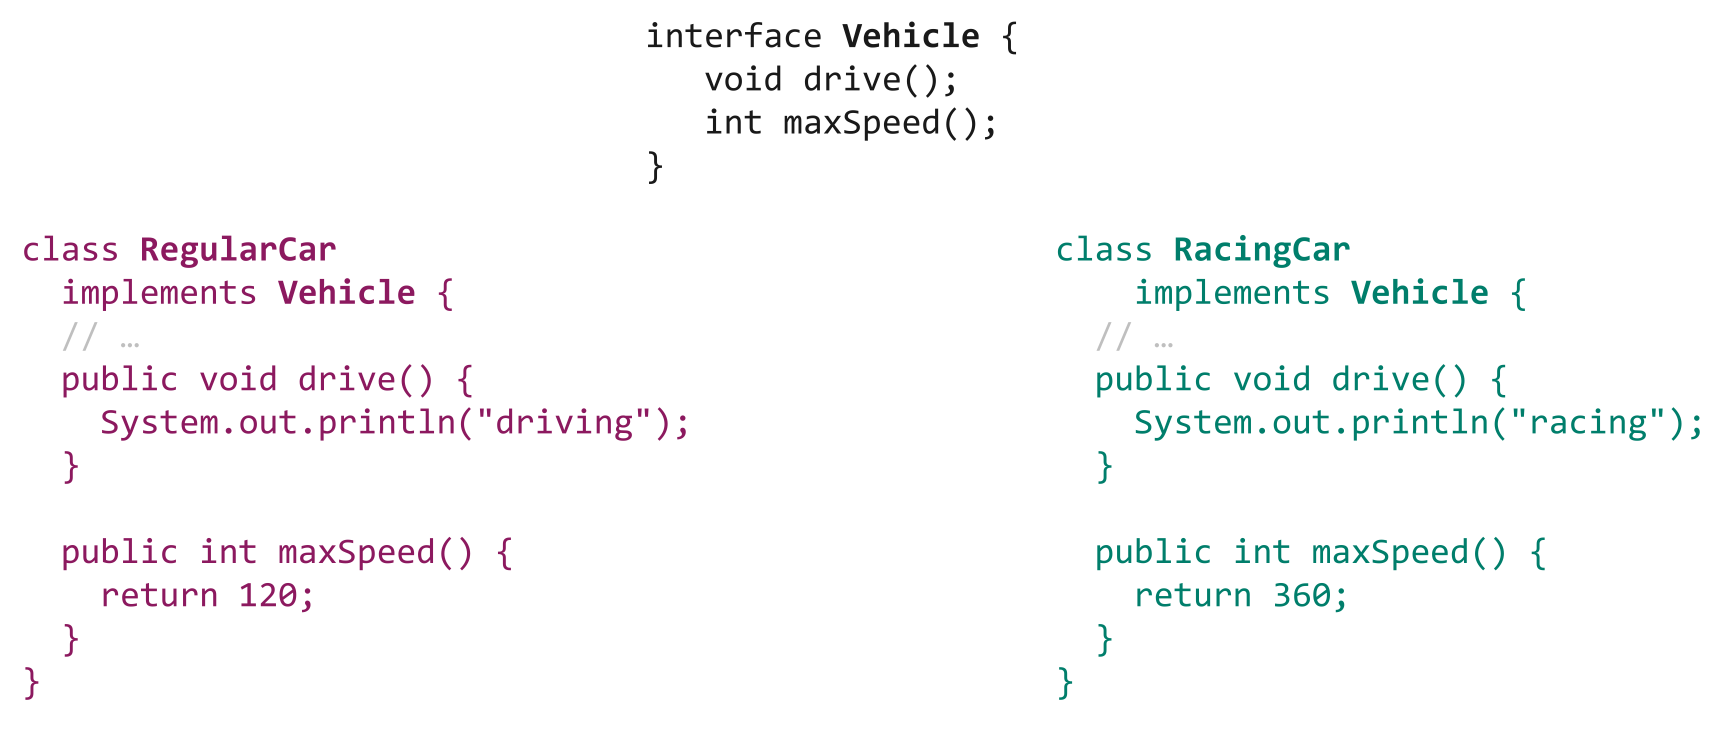
\includegraphics[width=0.9\columnwidth]{pictures/interface1-class2.png}
\end{center}

\subsection{Mehrere Interfaces - eine Implementierung}
\begin{center}
    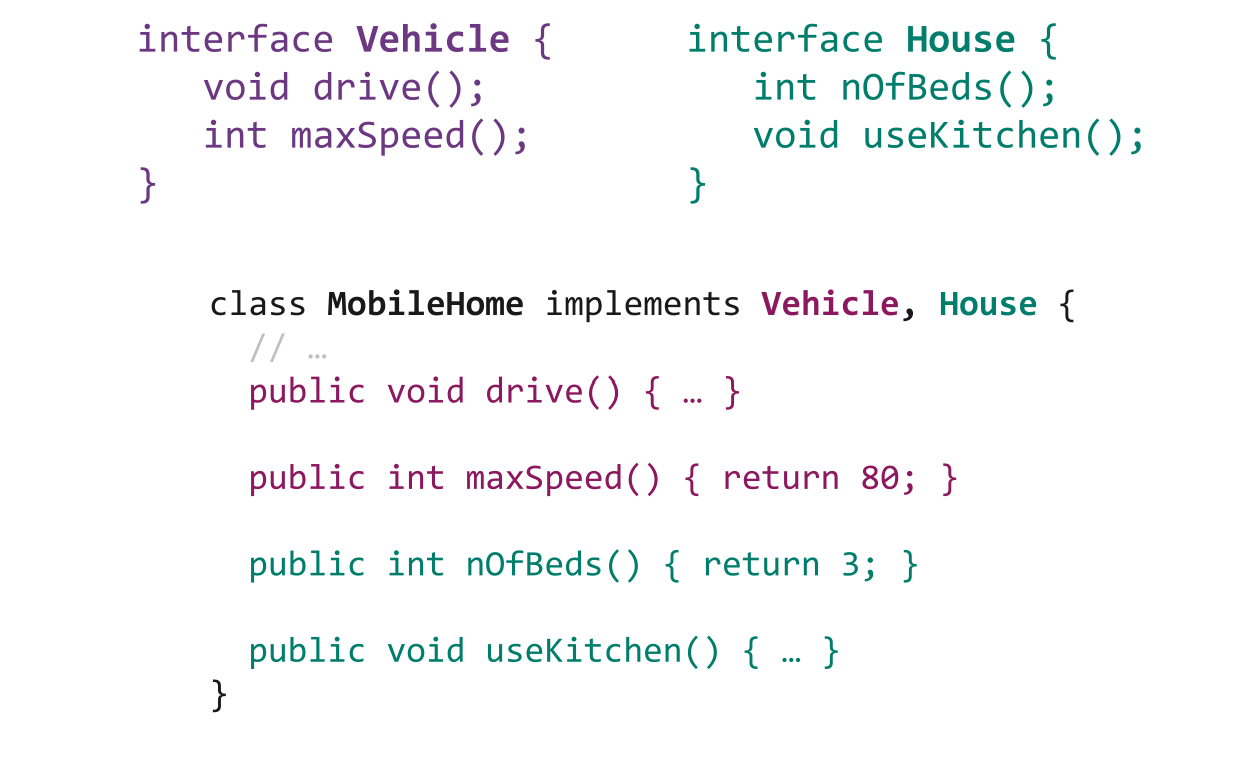
\includegraphics[width=0.9\columnwidth]{pictures/interface2-class1.png}
\end{center}